\chapter{Introduction}
\label{cha:introduction}

For a machine to interact in an intelligent manner with its outside world it needs to be
equipped with knowledge about it.  The very same is true for humans, and acquiring this
knowledge is a highly complex task which up to today is not completely understood.  To
help within this process, previously acquired knowledge is \emph{represented} in different
ways, \eg as books or films, to help others learning it.

However, the way knowledge is represented for human consumption is almost always not
suitable for machines.  While humans can extract knowledge from natural language, which
may be full of \emph{ambiguity}, machines require precise formulations of knowledge.  The
representation of knowledge in a machine-understandable way is the main focus of the area
of \emph{knowledge representation}~\cite{KRhandbook}.

One of the most successful approaches to knowledge representations are description
logics~\cite{DLhandbook}, a family of logic-based knowledge representations formalisms
with varying expressivity and reasoning complexity.  Description logics allow to represent
knowledge as \emph{knowledge bases} or \emph{ontologies}.  Essentially, these are just
collections of axioms, which may be either \emph{assertional} or \emph{terminological}.
For example, to represent the fact (the \emph{assertion}) that an individual \textsf{tom}
is a cat, one can use the assertional axiom
\begin{equation}
  \label{eq:14}
  \mathsf{Cat}(\mathsf{tom}).
\end{equation}
On the other hand, to state the terminological knowledge that every cat hunts mice, one
can use so-called \emph{general concept inclusions} and write
\begin{equation}
  \label{eq:15}
  \mathsf{Cat} \sqsubseteq \exists \mathsf{hunts}. \mathsf{Mouse}.
\end{equation}
As soon as a knowledge base is available, it is possible to \emph{reason} with it, \ie to
extract knowledge which is implicitly contained in this knowledge base.  For example, from
the two axioms state above, we can infer that the individual \textsf{tom} hunts mice.

Knowledge bases could be used to represent knowledge in a machine-consumable way.
However, the questions arises how to obtain such knowledge bases.  In one way or the
other, knowledge which is available to humans has to be translated into the form of a
description logic knowledge base.  Of course, this could be done by humans, but this
approach would not only be rather time-consuming but also prone to errors.  An automatic
translations would thus be highly welcome.  On the other hand, such an automatic
translation would just mean that machines can consume knowledge in the way humans
represent it, an assumption which is not reasonable.

However, one can still think about approaches which are \emph{semi-automatic} in the sense
that the results obtained from such a translation are preliminary and require further
refinement, or that the translation procedure requires additional \emph{assistance} by
means of human experts.

An approach to achieve such a semi-automatic translation procedure, or \emph{learning
  procedure}, has been made in~\cite{Diss-Felix}.  There, the focus lied in extracting
terminological knowledge of the form as given in \Cref{eq:14} from some given \emph{finite
  interpretation} $\mathcal{I}$.  More precisely, the procedures described
in~\cite{Diss-Felix} would automatically learn all general concept inclusions which are
\emph{valid} in the data set $\mathcal{I}$.  This approach made use of the mathematical
theory of \emph{formal concept analysis}, a subfield of mathematical order theory which
has very closed connections to description logics.

Of course, the general concept inclusions learned this way may not be correct, in the
sense that the general concept inclusion may hold in $\mathcal{I}$, but this data missed
to contain some relevant counterexamples.  One way to remedy this is to use an algorithm
from the field of formal concept analysis which is called \emph{attribute exploration}.
Within this algorithm, an expert (possibly human) is asked extracted general concept
inclusions for there correctness, and if proposed general concept inclusions are not found
then the expert has to provide \emph{counterexamples} to them.  This way, the problem that
the data may be \emph{incomplete} in that it lacks crucial counterexamples can be solved.
This has also been done in~\cite{Diss-Felix}.

However, there are still problems with this approach, especially if it comes to the
\emph{quality} of the data $\mathcal{I}$ from which general concept inclusions are
learned.  The main problem here is that the data may contain \emph{errors}.  These errors
may either cause otherwise valid general concept inclusions not to be found, because these
errors act as \emph{false counterexamples}, or general concept inclusions are found which
are not correct because errors cause positive counterexamples to vanish.  While the latter
approach can in theory be handled by the attribute exploration approach sketched above,
the former cannot, because the approach discussed in~\cite{Diss-Felix} will not even
extract general concept inclusions for which there may be errors in $\mathcal{I}$.

In this work, we want to extent the results obtain in~\cite{Diss-Felix} to this new
setting of where the data from which general concept inclusions are learned may contain
errors.  The main approach for this is to transfer the notion of
\emph{confidence}~\cite{arules:agrawal:association-rules} from the area of data-mining to
general concept inclusions.  Intuitively, this means that general concept inclusions may
have \emph{few} errors in the data, as opposed to having none in the original approach
of~\cite{Diss-Felix}.  The notion of ``few'' is quantified by means of the confidence of
the general concept inclusions in the data.

In the following we shall give a more in-depth overview of the problem sketched above, by
briefly introducing description logics and formal concept analysis in
Sections~\ref{sec:repr-knowl-using} and~\ref{sec:learn-impl-using}, respectively.  These
introductions will be mostly historical and by means of examples.  Thereafter, we discuss
in more detail what it means to learn general concept inclusions from data, and sketch our
approach of utilizing the notion of confidence to handle errors in the data.  This will be
done in Section~\ref{sec:extr-term-knowl}.  Finally, in Section~\ref{sec:related-work}, we
briefly discuss some related work which is important for our approach, and we summarize
our contribution in Section~\ref{sec:contributions}.

\section{Description Logics}
\label{sec:repr-knowl-using}

Description logics~\cite{DLhandbook} are a family of logic-based knowledge representation
formalisms, with a strong emphasis on well-defined semantics and practical reasoning
procedures.  The family of description logics contains various flavors of logical
formalisms, varying in expressiveness and reasoning complexity, allowing users to choose
the expressiveness they need, or the complexity they can afford, in their respective
applications.

The development of description logics~\cite{baader01overview} was motivated by earlier
knowledge representation formalisms like \emph{semantic networks}~\cite{SemanticNetworks}
or \emph{frame}~\cite{Minsky-Frames}, whose semantics was highly ambiguous, and mostly
depended on human interpretation or implementation details.  The need for well-defined and
predictable knowledge representation formalisms then lead to the first logic-based
systems~\cite{journals/cogsci/BrachmanS85}, which were, however,
incomplete~\cite{conf/kr/Schmidt-Schauss89}.

The term \enquote{description} in \enquote{description logics} is motivated by the
intention to use description logics to express knowledge about \emph{concepts
  descriptions}.  For this, description logics provide a number of constructors, which can
then be used to build concept descriptions from atomic \emph{concept names} and binary
\emph{role names}.  Then, two classical \emph{reasoning problems} are \emph{instance
  checking} and \emph{subsumption}: given an element $a$ and a concept description $C$,
the instance checking problem is to ask whether $a$ is an \emph{instance} of $C$, \ie
whether $a$ \emph{satisfies} the concept description $C$.  This can made more precise
using the notion of \emph{interpretations}, which are used more generally to define the
semantics of description logics.  Moreover, the subsumption problem is, given two concept
descriptions $C, D$, to ask whether it is true that $C$ is a \emph{subconcept} of $D$, \ie
whether every instance of $C$ is also an instance of $D$.

The first description logics considered were relatively small fragments of first order
logic, but already for them it could be shown that reasoning is
intractable~\cite{conf/aaai/BrachmanL84,journals/ai/Nebel88}.  One approach to remedy this
was to investigate highly optimized reasoning algorithms, which behave well in practice.
The most prominent class of such algorithms are \emph{tableau algorithms}, first invented
for the description logic
$\ALC$~\cite{journals/ai/Schmidt-SchaussS91,conf/ecai/HollunderNS90} for the subsumption
problem, and thereafter extended to other, even more expressive logics.  After a
connection of $\ALC$ to multimodal logic $\mathsf{K}_{(\mathsf{m})}$ was
discovered~\cite{DBLP:conf/ijcai/Schild91}, it was seen that this tableau algorithm is
actually a re-invention of the tableau algorithms used in modal logics.  The development
of description logics continued to investigate highly expressive description logics, whose
expressiveness exceeds that of $\ALC$, but which still behave well in
practice~\cite{journals/igpl/HorrocksST00}, and for which highly-optimized implementations
exist~\cite{sirin_pellet:practical_2007,Haarslev:2001,DBLP:conf/cade/TsarkovH06}.  This
finally lead to the adoption by the W3C of the \emph{Web Ontology Language OWL}, which is
based on the highly expressive description logic
$\mathcal{S}\mathcal{H}\mathcal{O}\mathcal{I}\mathcal{N}$~\cite{horrocks03fromshiqrdftoowl}.

The focus of description logics research departed from the sole focus on expressive
description logics when it was discovered at the beginning of this millennium that for the
in inexpressive description logic $\EL$ reasoning is
tractable~\cite{DBLP:conf/ijcai/Baader03a,DBLP:conf/ecai/Brandt04}, and stays polynomial
if the expressiveness of $\EL$ is extended
slightly~\cite{DBLP:conf/ijcai/BaaderBL05,BaaderEtAl-OWLED08DC}.  The practical relevance
of these results is given by the fact that large biomedical ontologies can be reformulated
as \emph{description logic knowledge bases} (or \emph{description logic ontologies}) using
just $\EL$ or a slight extension of it.  Examples for this are the \emph{Systematized
  Nomenclature of Medicine--Clinical Terms}, the Gene Ontology~\cite{gene-ontology}, and
large parts of the GALEN ontology~\cite{Rector199475}.

The main constructors of $\EL$ are conjunction ($\sqcap$) and existential restriction
($\exists$), and examples of $\EL$ concept descriptions are
\begin{equation*}
  \mathsf{Cat},\, \mathsf{Cat} \sqcap \mathsf{Mouse},\, \exists \mathsf{hunts}. \mathsf{Mouse}.
\end{equation*}
A description logic knowledge base formulated in $\EL$ usually consist, as any description
logic knowledge base, of two parts, namely an \emph{ABox}, holding assertional knowledge,
and a \emph{TBox}, containing terminological knowledge.  An example knowledge base would
then be
\begin{equation*}
  \mathcal{K} = (\set{ \mathsf{Cat} \sqsubseteq \exists \mathsf{hunts}. \mathsf{Mouse} },
  \set{ \mathsf{Cat}(\mathsf{tom}) }),
\end{equation*}
where the first entry denotes the TBox, and the second one denotes the ABox.

The semantics of knowledge bases is defined using \emph{interpretations} $\mathcal{I}$,
which can be thought of as edge- and vertex-labeled graphs.  The labels of the vertices,
which we shall \emph{elements} or \emph{individuals}, are concept names, and the labels of
the edges are role names.  An interpretation is a model of a knowledge base if all
elements satisfy the axioms contained in this knowledge base.  For example, the
interpretation
\begin{center}
  \begin{tikzpicture}[>=stealth']
    \begin{scope}[every node/.style = { draw, circle }]
      \node (Tom) {\textsf{tom}};
      \node[right=2cm of Tom, inner sep = .1cm] (Jerry) {\textsf{jerry}}; % fix
    \end{scope}
    \path (Tom) edge[->, bend left=30] node[midway, above] {\textsf{hunts}} (Jerry);
    \path (Jerry) edge[->, bend left=30] node[midway, below] {\textsf{hunts}} (Tom);
  \end{tikzpicture}
\end{center}
is a model of the knowledge base $\mathcal{K}$, since the element \textsf{tom} is labeled
with \textsf{Cat}, and every element which is labeled with \textsf{Cat} is connected to
some element labeled with \textsf{Mouse} via an edge labeled with \textsf{hunts}.

\section{Formal Concept Analysis}
\label{sec:learn-impl-using}

Formal concept analysis~\cite{fca-book} is a subfield of mathematical order theory,
originally concerned with the study of properties of ordered structures called
\emph{complete lattices} by representing them in terms of so-called \emph{formal
  contexts}.  However, since then, this theory has evolved into a rich field, with
connections to previously unrelated subjects such as
logics~\cite{books/math/Prediger00,conf/iccs/FerreR00}, data
mining~\cite{arules:Zaki:1998}, machine learning~\cite{conf/icfca/Kuznetsov04}, and
artificial intelligence~\cite{rudolph2006relational,Diss-Felix}.  Because of this, formal
concept analysis today can also be considered as a part of theoretical computer science,
and thus provides another link between this compute science and mathematics.

The origin of formal concept analysis as it is used in this work can clearly be marked by
the work of Wille~\cite{fca:Wille:1982}, which introduced formal concept analysis as an
approach to impose meaning on complete lattices as \emph{hierarchies of concepts}.  This
work was motivated by previous results from Birkhoff~\cite{books/math/Birkhoff67}, but
also has a strong philosophical background~\cite{books/phil/Hentig72}, see
also~\cite{Wille:Begriffsdenken}.  Another early work that included some of the ideas of
formal concept analysis is~\cite{OrdreEtClassification}.

The fundamental idea of formal concept analysis is to represent complete lattices by a
\emph{object-attribute-relationship}, which is expressed using \emph{formal contexts}.
These structures can be thought of as tables of crosses, like the following (taken
from~\cite{fca:Wille:1982})
\begin{equation*}
  \begin{array}[c]{c|*{7}{c}}
    \toprule
    ~       & \mathsf{small} & \mathsf{medium} & \mathsf{large} & \mathsf{inner} &
    \mathsf{outer} & \mathsf{moon} & \mathsf{no moon} \\
    \midrule
    \mathsf{Mercury} & \times &   &   & \times &   &   & \times  \\
    \mathsf{Venus}   & \times &   &   & \times &   &   & \times  \\
    \mathsf{Earth}   & \times &   &   & \times &   & \times &    \\
    \mathsf{Mars}    & \times &   &   & \times &   & \times &    \\
    \mathsf{Jupiter} &   &   & \times &   & \times & \times &    \\
    \mathsf{Saturn}  &   &   & \times &   & \times & \times &    \\
    \mathsf{Uranus}  &   & \times &   &   & \times & \times &    \\
    \mathsf{Neptune} &   & \times &   &   & \times & \times &    \\
    \mathsf{Pluto}   & \times &   &   &   & \times & \times &    \\
    \bottomrule
  \end{array}
\end{equation*}
This formal context expresses an object-attribute-relationship between the known planets
of the solar system (including Pluto) as \emph{objects}, and the \emph{attributes} whether
a planet is \textsf{small}, \textsf{medium}, or \textsf{large}, whether a planet is an
\textsf{inner} planet (\ie has an orbit which is closer to the sun than the asteroid
belt), or is an \textsf{outer} planet, and whether a planet has a \textsf{moon} or not.  A
cross in this table then means that the object on the corresponding row \emph{has} the
attribute on the corresponding column.  Thus, for example, \textsf{Mercury} is a
\textsf{small} planet, and \textsf{Pluto} is an \textsf{outer} planet.  The set of all
pairs of objects $g$ and attributes $m$ where $g$ has the attribute $m$ is called the
\emph{incidence relation} of the formal context.

From such a formal context one can then extract \emph{formal concepts}, which can be
ordered in a natural way to yield the \emph{concept lattice} of the formal context.  In
our example above, a formal concept which corresponds to the concept of a
\emph{medium-sized planet in our known solar system} would be the tuple
\begin{equation}
  \label{eq:60}
  ( \set{ \mathsf{Uranus}, \mathsf{Neptune} }, \set{ \mathsf{medium}, \mathsf{moon},
    \mathsf{outer} } ),
\end{equation}
where the first set is called the \emph{extent}, and the second set is called the
\emph{intent} of the formal concept.  Formal concept can then be ordered by set-inclusion
of their extents, and the concept lattice that corresponds to our small example above is
shown in \ref{fig:example-concept-lattice}.  This diagram also uses the usual, abridged
annotation of concept lattices: a node $v$ in the lattice diagram represents the formal
concept whose extent consists of all objects which can be reached by an \emph{descending
  path} in the diagram, starting from $v$.  Likewise, the intent of $v$ is the set of all
attributes that can be reached by an \emph{ascending path} in the diagram, starting from
$v$.  Thus, the gray-shaded node in \Cref{fig:example-concept-lattice} is the formal
concept of \Cref{eq:60}.

\begin{figure}[tp]
  \tikzset{vertexbase/.style={semithick, shape=circle, inner sep=2pt, outer sep=0pt, draw},%
    vertex/.style={vertexbase},%
    mivertex/.style={vertexbase},%
    jivertex/.style={vertexbase},%
    divertex/.style={vertexbase},%
    conn/.style={-, thick}%
  }
  \begin{center}
    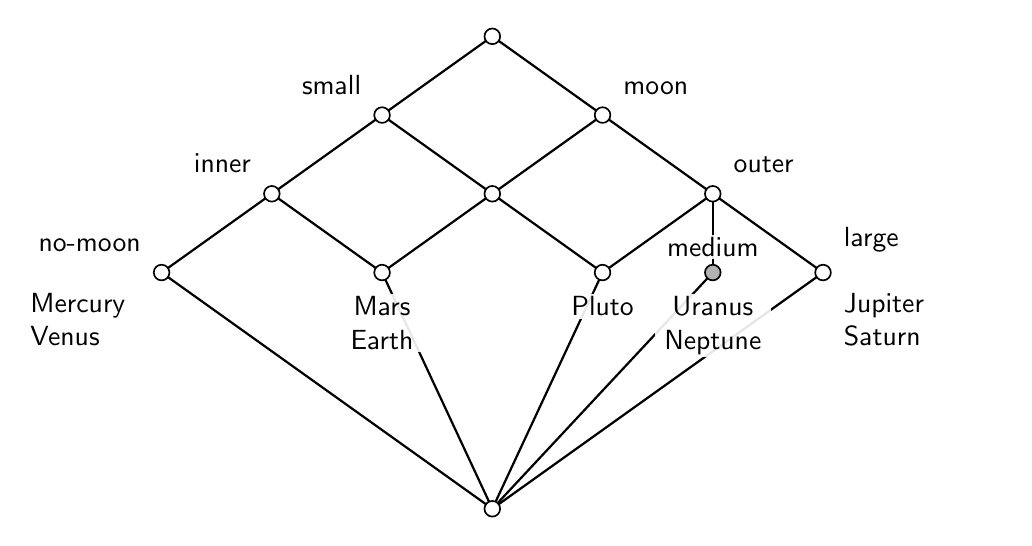
\begin{tikzpicture}
      \begin{scope}[xscale=.7] %for scaling and the like
        \begin{scope} %draw vertices
          \foreach \nodename/\nodetype/\xpos/\ypos in {%
            0/vertex/2/4,
            1/divertex/-4/7,
            2/jivertex/0/7,
            3/divertex/8/7,
            5/jivertex/4/7,
            6/mivertex/-2/8,
            7/vertex/2/8,
            8/mivertex/6/8,
            9/mivertex/0/9,
            10/mivertex/4/9,
            11/vertex/2/10
          } \node[\nodetype] (\nodename) at (\xpos, \ypos) {};
          \node[divertex,fill=black!30] (4) at (6,7) {};
        \end{scope}
        \begin{scope} %draw connections
          \path (7) edge[conn] (10);
          \path (9) edge[conn] (11);
          \path (5) edge[conn] (8);
          \path (1) edge[conn] (6);
          \path (0) edge[conn] (4);
          \path (0) edge[conn] (3);
          \path (8) edge[conn] (10);
          \path (5) edge[conn] (7);
          \path (6) edge[conn] (9);
          \path (2) edge[conn] (7);
          \path (0) edge[conn] (1);
          \path (3) edge[conn] (8);
          \path (2) edge[conn] (6);
          \path (10) edge[conn] (11);
          \path (7) edge[conn] (9);
          \path (4) edge[conn] (8);
          \path (0) edge[conn] (2);
          \path (0) edge[conn] (5);
        \end{scope}
        \begin{scope}[every label/.style={font=\sffamily, inner sep=1pt, fill opacity=.9,
            text opacity=1, fill=white, label distance=4pt}] %add labels
          \foreach \nodename/\labelpos/\labelopts/\labelcontent in {%
            1/below left//{\parbox{1.4cm}{Mercury\\ Venus}},
            1/above left//{no-moon},
            2/below//{\parbox{2cm}{\centering Mars\\ Earth}},
            3/below right//{\parbox{2cm}{Jupiter\\ Saturn}},
            3/above right//{large},
            4/below//{\parbox{1.4cm}{\centering Uranus\\ Neptune}},
            5/below//{Pluto},
            6/above left//{inner},
            8/above right//{outer},
            9/above left//{small},
            10/above right//{moon}
          } \node[draw=none,label={[\labelopts]\labelpos:{\labelcontent}}] at (\nodename) {};
          \node[draw=none,label={[label distance=1pt]above:medium}] at (4) {};
        \end{scope}
      \end{scope}
    \end{tikzpicture}
  \end{center}
  \caption{Example Concept Lattice}
  \label{fig:example-concept-lattice}
\end{figure}

One of the key results of formal concepts analysis is that every complete lattice can be
represented as a concept lattice of a suitably chosen formal context (the so-called
\emph{fundamental theorem of formal concept analysis}).  A major direction of formal
concept analysis research is now to consider properties and operations of lattices, such
as distributivity, modularity, direct and semi-direct products, and transfer them to
corresponding properties and operations on the level of formal contexts.
See~\cite{fca-book} for more details on this.

Another very prominent research direction is the study of \emph{implications} in formal
contexts, which has been discussed as early as~\cite{fca:Wille:1982}.  Observe that in our
example formal context above, all outer planets have a moon.  We can express this fact as
saying that the implication
\begin{equation*}
  \set{ \mathsf{outer} } \to \set{ \mathsf{moon} }
\end{equation*}
\emph{holds} in our formal context.  Implications are similar to \emph{functional
  dependencies} from the theory of databases~\cite{DBLP:books/cs/Maier83}, and also play a
certain role in classical order theory~\cite{Wild1994118}.

One task is then to compute the set of all valid implications of a given formal context.
Since this set can be quite huge, one usually wants to compute \enquote{small} sets of
implications which are sufficient, called \emph{bases}.  One very prominent base is the
so-called \emph{canonical base}~\cite{fca:DuquenneGuigues:1986} (also \emph{stem base},
\emph{Duquenne-Guigues base}), which is a \emph{minimal} base, \ie a base with minimal
cardinality.  This base can be computed
effectively~\cite{DBLP:conf/icfca/Ganter10,DBLP:journals/amai/ObiedkovD07}, however these
algorithms not efficient~\cite{DBLP:conf/icfca/Distel10} with respect to size of the input
and the output.  Certain complexity results suggest that efficiently computing the
canonical base is not possible in general~\cite{DBLP:journals/dam/BabinK13}.  However, if
this is really the case is an open research question.  Therefore, other bases have been
investigated, whose computation is algorithmically easier.  An example is the base of
\emph{proper premises}~\cite{fca-book}, for which fast algorithms
exist~\cite{RyDiBo-AMAI13}.

An algorithm which is related to the study of valid implications of formal contexts is
\emph{attribute exploration}~\cite{fca-book,GORS-book}, which is an interactive process
which extracts valid implications from \emph{incomplete} data utilizing \emph{expert
  interaction} to obtain missing facts.  Within this process, an external expert is asked
questions of the form
\begin{equation*}
  \text{Is the implication } A \to B \text{ valid?}
\end{equation*}
The expert can the either accept this implication, or decline it by providing a
\emph{counterexample}.  In this way, the expert enriches the currently known formal
context by missing objects and their attributes.  As soon as the process finishes, the set
of confirmed implications represents the whole implicational knowledge represented by the
expert, and it indeed be shown that this set of confirmed implications is the canonical
base of the formal context which is constituted by all counterexamples provided by the
expert.  In this way, attribute exploration can be seen as an semi-automatic knowledge
acquisition algorithm.

Attribute exploration has been a major focus of formal concept analysis, and many
extensions of this algorithm have been developed and discussed.  Examples for this are the
inclusion of \emph{background
  knowledge}~\cite{stumme96attribute,DBLP:journals/tcs/Ganter99}, \emph{concept
  exploration}~\cite{conf/iccs/Stumme97}, \emph{rule
  exploration}~\cite{phd/de/Zickwolff1991}, \emph{relational
  exploration}~\cite{rudolph2006relational}, exploration in the presence of \emph{partial
  knowledge}~\cite{DBLP:conf/fca/BurmeisterH05,BGSS07}, and \emph{model
  exploration}~\cite{Diss-Felix}.

\section{Extracting Terminological Knowledge from Relational Data}
\label{sec:extr-term-knowl}

The main purpose of this work is to discuss a way to extract general concept inclusions
from relational data (interpretations) which are allowed to contain \enquote{few} errors.
The basis for our considerations are the results obtained by Baader and
Distel~\cite{Diss-Felix,BaDi09,BaaderDistel08} on computing \emph{finite bases} of
\emph{valid} general concept inclusions from finite interpretations.

For this approach we assume that we want to learn terminological knowledge about a certain
\emph{domain} of interest, and that we can represent this domain as a finite
interpretation $\mathcal{I}$.  In other words, our domain is representable as relational
data, where the elements have additional properties.  Then the terminological knowledge we
are interested in is exactly the set $\Th(\mathcal{I})$ of valid general concept
inclusions of $\mathcal{I}$, in our case using the description logic $\ELbot$.

A first problem here is that the set $\Th(\mathcal{I})$ is infinite in general: if $C
\sqsubseteq D$ is valid in $\mathcal{I}$, and if $r$ is a role name, then the general
concept inclusion $\exists r. C \sqsubseteq \exists r. D$ is also valid in $\mathcal{I}$.
To remedy this, Baader and Distel want to compute \emph{finite bases} of
$\Th(\mathcal{I})$, \ie finite subsets of $\Th(\mathcal{I})$ which are already complete
for $\mathcal{I}$.  One of the main results of their approach is then that such finite
bases always exist, and that they can be computed effectively.  Such finite bases can then
be used as TBoxes of a knowledge base which logically represents the initial domain of
interest.

To provide these results, Baader and Distel exploit the tight connection between the
description logic $\ELbot$ and formal concept analysis which is established by \emph{model
  based most specific concept descriptions} and \emph{induced formal contexts} of finite
interpretations and sets of concept descriptions.  More precisely, it can be shown that if
$\con K_{\mathcal{I}}$ denotes the induced formal context of $\mathcal{I}$, that then
every base of $\con K_{\mathcal{I}}$ gives rise to a finite base of $\mathcal{I}$.
Moreover, it is possible to transfer the algorithm of attribute exploration applied to the
context $\con K_{\mathcal{I}}$ to an algorithm for \emph{model exploration} of
$\mathcal{I}$.  This algorithm then allows to interactively compute bases of
$\mathcal{I}$, allowing an expert to provide missing facts when required.  The resulting
algorithms obtain by this approach are all effective, and can be implemented.  This has
been done in a preliminary version in~\cite{DBLP:conf/icdm/BorchmannD11}.

\section{Other Related Work}
\label{sec:related-work}

The work of Baader and Distel is not the first attempt to bring together the worlds of
description logics and formal concept analysis.  Indeed, there have been several previous
attempts to utilize formal concept analysis for description logic applications, and to add
ideas from description logics to notions of formal concepts analysis.

One of the first results in description logics that utilizes formal concept analysis is
the work of Baader~\cite{Baader-KRUSE-95}.  In this work, Baader uses the attribute
exploration algorithm on a special formal context to compute a minimal representation of
the subsumption hierarchy between all conjunctions of the defined concept names of a given
acyclic TBox $\mathcal{T}$, formulated in the logic $\ALC$.  To this end, Baader extends
the classical algorithm~\cite{journals/ai/Schmidt-SchaussS91} for \ALC to decide
subsumption between \emph{single} defined concept names, and extends it in such a way that
it provides counterexamples to instances of the subsumption problem.  These
counterexamples are then collected into a suitable formal context, and from this context
the attribute exploration algorithm eventually computes the canonical base.  These
implications give rise to a set of general concept inclusions, which can then be used to
decide subsumption between conjunctions of defined concept names of $\mathcal{T}$.

The results obtained by Baader have been further generalized by
Stumme~\cite{stumme96concept} to include also disjunction.  For this, a generalization of
attribute exploration called \emph{distributive concept
  exploration}~\cite{conf/ki/Stumme98} is used.

Another use of ideas from formal concept analysis for description logic applications is in
\emph{knowledge base completion}~\cite{Sert07,BGSS07}, for which again attribute
exploration was used.  For this, GCIs of the form
\begin{equation*}
  \bigsqcap U \sqsubseteq \bigsqcap V
\end{equation*}
are asked to the expert, where $U, V \subseteq M$ for some previously chosen set $M$ of
interesting concepts.  The task is then to ensure the given knowledge base is complete
with respect to all these general concept inclusions, \ie the knowledge base should entail
all such general concept inclusions which are confirmed by the expert, and should contain
counterexamples for all other general concept inclusions of this type.  The most
significant challenge for transferring attribute exploration to this setting is to deal
with the \emph{open world semantics} of description logic knowledge bases: a fact that is
not stated in the knowledge base does not mean that the negated fact holds.  For this,
attribute exploration is generalized to work on \emph{partial contexts}, \ie formal
context in which certain crosses are unknown.  The resulting algorithm has been
implemented as a plugin named \emph{OntoComp} for the ontology editor
\emph{Protégé}~\cite{Sert09b}.

A third prominent application of ideas of formal concept analysis in description logics is
the work of Rudolph on \emph{relational
  exploration}~\cite{DBLP:phd/de/Rudolph2006,conf/iccs/Rudolph04}.  In this approach, the
target description logic is \FLE, the extension of \EL by value restriction ($\forall$).
The domain of interest is not represented as an interpretation, but by means of
\emph{binary power context families}~\cite{DBLP:conf/iccs/PredigerW99}, which however can
easily be considered as an interpretation.  Then the exploration process is conducted in
several phases: in phase $k$, concept descriptions with \emph{role depth} at most $k$ are
considered as attributes of the current formal context, and on this formal context
attribute exploration is performed.  Rudolph then shows that this process has only to be
considered up to a certain maximal role depth, and that the resulting set of implications
can be used to decide whether an arbitrary general concept inclusion $C \sqsubseteq D$ is
valid in the original domain or not.  However, it is not shown whether and how this set of
implications can be transferred into a base of the domain.  Indeed, the decision procedure
for checking whether $C \sqsubseteq D$ holds in the domain or not is rather complicated.
Thus, no general concept inclusions are learned from this approach, and thus it cannot be
used to obtain terminological knowledge from relational data.

The aforementioned approach of binary power context families is an attempt to add
description logic expressibility to the world of formal concept analysis.  In its easiest
form, \emph{relational contexts} (also \emph{binary power context families}), a formal
context is equipped with a family of relations $\mathcal{R}$ on the object set.  Based on
this notion, \emph{terminological attribute logic}~\cite{books/math/Prediger00} has been
introduced that allows to define new attributes in terms of old ones, using the relational
context to extend the incidence relation to the newly defined attributes.  With this
semantics, terminological attribute logic can be seen as a syntactic variant of the of
\ALC extended by inverse roles, negated roles and the identity role.

\todo[inline]{Write: previous connections between FCA and DL (RCA)}%
\todo[inline]{Write: mention Luxenburger}%
\todo[inline]{Write: mention Fuzzy-FCA and Fuzzy-DL, Vagueness in general}%

\section{Contributions}
\label{sec:contributions}

\todo[inline]{Write: say that obtaining an interpretation that faithfully represents a
  domain of interest is not possible in real applications}

\subsection{Experiments with Extracting Valid GCIs}
\label{sec:exper-with-extr}

\subsection{Extracting GCIs from Erroneous Data}
\label{sec:extracting-gcis-from}

\subsection{Exploration by Confidence}
\label{sec:expl-conf-2}

\subsection{Model-Exploration by Confidence with Completely Specified Counterexamples}
\label{sec:model-expl-conf}

\section{Acknowledgments}
\label{sec:acknowledgements}

\todo[inline]{Write: acknowledgments}

%%% Local Variables: 
%%% mode: latex
%%% TeX-master: "../main"
%%% End: 

%  LocalWords:  Protégé OntoComp
